\documentclass{article}

\PassOptionsToPackage{numbers,sort&compress}{natbib}
\usepackage[final,main]{neurips_2025}

\usepackage[utf8]{inputenc}
\usepackage[T1]{fontenc}
\usepackage{hyperref}
\usepackage{url}
\usepackage{booktabs}
\usepackage{amsfonts}
\usepackage{nicefrac}
\usepackage{microtype}
\usepackage{xcolor}
\usepackage{amsmath}
\usepackage{graphicx}
\usepackage{CJKutf8}

\title{Deep Learning Hint Agent: A Next-Action Decision Framework for Progressive Competitive Programming Hints}

% Double-blind review stage requires anonymous author formats.
% \author{%
%   Haikun Zhao 2025040161, Ninghuan Chen 2025040141   \\
%   Institute for Interdisciplinary Information Sciences (IIIS) \\
%   Tsinghua University \\
%   \texttt{zhk25@mails.tsinghua.edu.cn} \texttt{cnh25@mails.tsinghua.edu.cn} \\
% }

\author{%
  Team Leader \\
  \texttt{2025040161} \\
  \And
  Team Member 1 \\
  \texttt{2025040141} \\
}

\begin{document}

\begin{CJK*}{UTF8}{gbsn}

\maketitle

\begin{abstract}
  In competitive programming platforms like Codeforces, providing users with raw editorials or complete code directly often undermines the educational process. This paper presents a Deep Learning Hint Agent designed for progressive hint generation. Traditional attempts model full hint conversations as a single sequence, which forces the model to learn a statistical average hint length rather than adaptively terminating based on problem complexity. To resolve this, we reformulate hint generation as a \textbf{Next-Hint Decision Task}. By fine-tuning Qwen-Coder-7B \cite{qwen2024} using LoRA SFT, the agent evaluates the problem statement, the official editorial, and the hints generated so far to independently decide the next optimal local action: output a brand new pedagogical hint or stop the process. To resolve the zero-shot baseline pitfalls of semantic repetition and early cutoff, we introduce synthetic negative rejection datasets, a multi-candidate inference reranking pipeline, and an abbreviated training cycle. Our evaluations using an external solver show that the progressive hints significantly guide problem-solving steps while maintaining the concise, punchy brevity characteristic of the Codeforces community \cite{codeforces2023}.
\end{abstract}

\section{Introduction}
Providing scalable, high-quality hints for complex algorithmic problems remains a challenge for general large language models (LLMs). When prompted in a zero-shot manner, state-of-the-art models default to static formatting architectures regardless of the actual problem difficulty, often inadvertently giving away key algorithmic formulations or code blocks prematurely \cite{codeforces2023}.

Rather than training a model to predict an entire sequence of multi-turn dialogues, our project treats progressive hint generation as a \textbf{Conditional Next-Action Policy}. At each individual iteration step, the model observes the current local hint state and determines whether the user requires another step of intuition or if the gap left is merely implementation work. This mimics the strategic, progressive scaffolding provided by real human coaches in competitive programming environments.

\section{Data Collection and Processing}

\subsection{Scraping and Cloudflare Access Control}
Compiling a clean dataset of official problem statements and corresponding hints directly from Codeforces is restricted by aggressive security configurations. Scraping direct problem statement pages repeatedly triggers Cloudflare access blocks. Through exploratory access testing, we observed that Codeforces \textbf{contest pages} and \textbf{editorial blog pages} maintain significantly lighter protective parameters.

Consequently, we constructed a distributed scraper utilizing multiple data origins:
\begin{itemize}
    \item \textbf{Codeforces Contest Pages:} Used exclusively to extract clean problem metadata, hyperlinks, and target problem names.
    \item \textbf{Codeforces Editorial/Blog Pages:} Used to pull the native official tutorial content and baseline hint sequences.
    \item \textbf{Luogu Mirror Pages:} Utilized to map and fetch the raw Codeforces problem statements safely without hammering protected source endpoints.
\end{itemize}
Conservative, randomized query sleep intervals were implemented throughout the entire scraping runtime to guarantee pipeline stability and eliminate request throttling.

\subsection{Dynamic Editorial Loading Resolution}
During the processing of Codeforces editorial blogs, pages occasionally render a transient \texttt{[Tutorial is loading...]} placeholder script. If captured naively, the dataset becomes poisoned with empty text strings. Our scraper handles this through an integrated automated retry block, pausing and forcing re-fetches until the real DOM contents are successfully populated.

\subsection{Dataset Structure}
The raw outputs are segmented into two localized directory structures: \texttt{with\_hint/} and \texttt{without\_hint/}. A validated JSON payload adheres to the following structural topology:
\begin{verbatim}
{
  "statement": [{"title": "Statement", "content": "..."}],
  "hints":     [{"content": "..."}],
  "solutions": [{"title": "Solution", "content": "..."}]
}
\end{verbatim}

\section{Core Formulation}
Let a complete progressive hint sequence for an algorithmic challenge be denoted as $H_1, H_2, H_3, \dots, H_m$. Instead of modeling the complete string array as a unified continuous context, we structure the multi-turn sequence into isolated supervised training iterations.

The state-conditioned next-hint SFT examples are mapped out as follows:
\begin{itemize}
    \item \textbf{Turn 1 Input:} Statement + Editorial + No Previous Hints $\rightarrow$ \textbf{Output:} $H_1$ (Reveal the most preliminary observation).
    \item \textbf{Turn 2 Input:} Statement + Editorial + $H_1$ $\rightarrow$ \textbf{Output:} $H_2$ (Advance one small step beyond $H_1$).
    \item \textbf{Turn $k$ Input:} Statement + Editorial + $H_1 + \dots + H_{k-1}$ $\rightarrow$ \textbf{Output:} $H_k$.
    \item \textbf{Final Turn Input:} Statement + Editorial + $H_1 + H_2 + \dots + H_m$ $\rightarrow$ \textbf{Output:} \texttt{stop} (Cease generation when remaining steps are trivial implementation details).
\end{itemize}

Formally, the fine-tuned network approximates the local optimization policy function:
\begin{equation}
\text{Action}_{next} = f(\text{Statement}, \text{Editorial}, \{H_1, \dots, H_k\})
\end{equation}
where $\text{Action}_{next} \in \{\text{New Hint}, \texttt{stop}\}$.

\subsection{Structured Action Output Format}
Although the next-action policy can be abstractly written as a binary choice between generating a new hint and stopping, the actual SFT target is implemented as a structured JSON-style response. For a normal hint action, the model is trained to output:
\begin{verbatim}
{
  "action": "hint",
  "covered_so_far": ["short summary of previous hints"],
  "next_focus": "the next preliminary and critical observation",
  "hint": "**Hint k**\n..."
}
\end{verbatim}
For a stopping action, the corresponding target format is:
\begin{verbatim}
{
  "action": "stop",
  "covered_so_far": ["short summary of previous hints"],
  "next_focus": "",
  "hint": "No. The rest you need to think about yourself."
}
\end{verbatim}

This schema forces the model to explicitly summarize what has already been covered and identify the next local pedagogical focus before producing the user-facing hint. In practice, this reduces uncontrolled free-form continuation and makes the generation behavior easier to validate during inference. The generated hint is expected to contain only the next smallest useful observation, rather than a complete algorithm or implementation.

\section{System Improvements}
To mitigate the dual structural failures of premature stopping and semantic near-duplication (e.g., repeating the same strategy using minor vocabulary shifts), we deploy three main system improvements.

\subsection{Expanded Synthetic Rejection Data}
The baseline dataset was expanded beyond pure ground-truth pathways to incorporate targeted synthetic negative cases (Table~\ref{tab:data_types}).

\begin{table}[h]
  \caption{Data Typologies and SFT Training Intentions}
  \label{tab:data_types}
  \centering
  \begin{tabular}{ll}
    \toprule
    Data Type & Explicit Training Intention \\
    \midrule
    \texttt{raw\_hint\_decision} & Learn normal Codeforces-style progressive next-hint flows. \\
    \texttt{synthetic\_early\_stop\_rejection} & Penalize early \texttt{stop} actions when core logical gaps remain. \\
    \texttt{synthetic\_repeat\_rejection} & Suppress semantic near-duplicates and discourage circular hints. \\
    \bottomrule
  \end{tabular}
\end{table}

\subsection{Candidate Inference Generation and Reranking}
During inference, the framework rejects single-token greedy sampling. Instead, the local model spawns $10$ discrete candidate decisions simultaneously. These vectors pass through a strict reranking evaluation script (Table~\ref{tab:rerank_logic}).

\begin{table}[h]
  \caption{Candidate Reranking Penalty Architecture}
  \label{tab:rerank_logic}
  \centering
  \begin{tabular}{ll}
    \toprule
    Case Triggered & Applied Heuristic Treatment \\
    \midrule
    \texttt{stop} Decision & Applies a moderate penalty to allow natural stops without hyper-aggression. \\
    Exact String Duplicate & Applies a structural veto-level penalty to drop the branch. \\
    Semantic Near-Duplicate & Measures a Jaccard similarity index across normalized text; scales penalty. \\
    Excessive Length & Imposes a character length penalty to enforce punchy, brief outputs. \\
    \bottomrule
  \end{tabular}
\end{table}

\subsection{Short-Epoch SFT Strategy}
Our empirical validations revealed that optimizing the loss function until complete convergence (taking approx. $800 \sim 1200$ epochs) led to deterministic over-fitting. Linguistic diversity dropped sharply, causing severe repetition behavior. Restricting the SFT lifecycle to an abbreviated window of $150 \sim 250$ epochs leaves adequate linguistic variations intact, lowering near-duplications significantly.

\section{Experiments and Baseline Analysis}

\subsection{Zero-Shot Performance Benchmarks}
To understand the baseline capability of un-tuned architectures, we ran a zero-shot comparative benchmark on 6 Codeforces problems spanning a broad complexity envelope (Ratings $800 \sim 3300$) \cite{codeforces2023}. We tested Gemini-3.1 Flash Lite, DeepSeek V3, Kimi K-2.5 Pro, and Qwen3.6-35B-A3B with an identical prompt format: \textit{``请生成codeforce风格hint''} \cite{codeforces2023}.

The resulting zero-shot outputs evaluated under a blind manual annotation scheme are detailed in Table~\ref{tab:baseline_metrics}.

\begin{table}[th]
  \caption{Zero-Shot Multi-Model Hint Performance Metrics \cite{codeforces2023}}
  \label{tab:baseline_metrics}
  \centering
  \resizebox{\textwidth}{!}{%
  \begin{tabular}{llllllll}
    \toprule
    Model & Hint Count & Hint Length & Direct Reveal (Formulas) & Granularity \& Detail & Scalability to Difficulty & Socratic Tone & Progressive Logic \\
    \midrule
    \textbf{Gemini 3.1 Flash Lite} & 4 (Low) & Excessively Long & Moderate & Overly Descriptive & Static & Low & Moderate \\
    \textbf{Qwen 3.6-35B-A3B} & 3 (Very Low) & Moderate & Low & Too Abstract/General & Static & Moderate & Moderate \\
    \textbf{DeepSeek V3} & 6 (Moderate) & Long & High (Frequent) & Instructional & Static & Low & High \\
    \textbf{Kimi K2.5 Pro} & 12 (Excessive) & Short  & Moderate & Overly Granular & Static & Low & High \\
    \bottomrule
  \end{tabular}%
  }
\end{table}

The zero-shot analysis exposes an overarching critical flaw: all tested baselines demonstrate an absence of difficulty-scaling awareness \cite{codeforces2023}. They deploy a static, uniform distribution of hints regardless of whether the problem is simple (Rating 800) or highly advanced (Rating 3300) \cite{codeforces2023}. Furthermore, their text tone is overly instructional, acting as step-by-step guides that give away the solution instead of providing subtle "nudges" to provoke critical thinking \cite{codeforces2023}. This highlights the necessity for specialized SFT tuning \cite{codeforces2023}.

\subsection{External Solver Evaluation Loop}
To quantify hint utility automatically, we built an evaluation sandbox. An external model (\textbf{DeepSeek V4-Pro}~\cite{deepseek_v4_preview}) is deployed as a proxy user. This solver attempts to generate valid C++ code under isolated condition matrices. 
To bypass editorial copy-pasting shortcuts, a dedicated script (\texttt{fix\_solution\_include\_and\_regenerate.py}) cleans official tutorial text inputs by dropping code components starting from the first \texttt{\#include} tag, replacing them with a \texttt{[code block omitted]} token.

\paragraph{Choice of Solver Model and Difficulty.}
We use a controlled evaluation setting with a fixed competitive-programming difficulty and a fixed external solver. Several freely available models were initially tested, but their competitive-programming ability was insufficient to create a meaningful intermediate evaluation range. We therefore selected \textbf{DeepSeek V4-Pro} as the proxy solver and fixed the benchmark difficulty to \textbf{Codeforces rating 1700}. Empirically, this setting creates a useful contrast: the solver is usually not reliable under the statement-only condition, but can solve many problems when provided with the cleaned official editorial. Consequently, generated hints can be evaluated as intermediate scaffolding signals between these two endpoints.

\paragraph{Evaluation Segment Construction.}

Because official programmatic submission is not available in our evaluation setting, all generated code is manually submitted to the Codeforces judging platform by our team. For a problem with $k$ generated hints $H_1, H_2, \dots, H_k$, we construct $k+2$ isolated solver conditions:

\begin{verbatim}
Hint0      : statement only
Hint1      : statement + H1
Hint2      : statement + H1 + H2
...
Hintk      : statement + H1 + H2 + ... + Hk
Solution   : statement + cleaned official editorial
\end{verbatim}

The official editorial is used only in the final \texttt{Solution} upper-bound condition and is not exposed to the solver during generated-hint evaluation. This design allows us to measure whether the accepted-code rate increases as progressively more model-generated hints are provided.

\paragraph{Manual AC Adjudication.}

For each condition, the solver-generated C++ file is submitted to Codeforces, and the final Accepted/Rejected outcome is recorded manually. Although this workflow is more labor-intensive than using a fully local judge, it directly matches the target platform's native judging behavior and avoids discrepancies caused by incomplete local test coverage.

The progressive state milestones are tracked via manual AC logs recorded as multi-bit strings (e.g., \texttt{CF1792D 0011111}). The first bit represents the base condition (Hint0, problem statement only), the middle positions track performance across sequential agent hints ($1 \sim k$), and the final index records upper-bound performance under the cleaned solution condition.


\subsection{Qualitative Example of Generated Hints}

To qualitatively inspect whether the trained agent produces progressive and non-redundant guidance, we present one representative generated hint sequence below. The hints are intentionally short and Codeforces-style: each step reveals only one additional observation, while avoiding direct implementation details. Below are the hint results generated by the model in CF2205D.

\begin{quote}
\textbf{Hint 1.}
The maximum number of each segment cannot be moved, and either the left side or the right side will be removed completely.

\textbf{Hint 2.}
The maximum number of both sides cannot be removed, either.

\textbf{Hint 3.}
A Cartesian Tree can be used.

\textbf{Hint 4.}
Any path from the root corresponds to a way to keep the maximum number on one side and delete the others.

\textbf{Hint 5.}
Calculate the depth of each node $d_u$, then the answer is $n - \max d_u$.
\end{quote}

This example illustrates the desired progressive behavior. The first two hints expose structural constraints about the maximum element without naming the full algorithm. The third hint introduces the key data structure, while the final hints connect the Cartesian tree representation to the final optimization objective. In this way, the agent gradually moves from local observations to the complete algorithmic insight.



\subsection{Fine-Tuned Model Empirical Results}
To evaluate the downstream utility of our progressive hint generator and examine the impact of conditioning parameters, we conduct a comparative benchmark across two training iterations of our agent. 

\begin{figure}[h]
  \centering
  \includegraphics[width=0.65\textwidth]{figure1.png}
  \caption{External solver coding accuracy across normalized hint progress before applying the hard truncation heuristic.}
  \label{fig:accuracy_uncapped}
\end{figure}

\begin{figure}[h]
  \centering
  \includegraphics[width=0.75\textwidth]{figure2.png}
  \caption{External solver coding accuracy after applying the four-hint truncation heuristic to Version 2.}
  \label{fig:accuracy_capped}
\end{figure}

\begin{itemize}
    \item \textbf{Version 1 (With solution hint generation):} In this variant, the full official solution/editorial is integrated directly into the context payload during the SFT training phase. As demonstrated in Figure~\ref{fig:accuracy_uncapped}, Version 1 achieves the strongest overall performance, starting from a baseline accuracy of $29.2\%$ at $0\%$ hint progress and gradually improving in aggregate despite several local drops to a peak accuracy of $53.3\%$ at approximately $88\%$ progress, tracking closely toward the official solution upper-bound of $77.1\%$. The overall upward trend suggests that the generated progressive hints provide useful conceptual guidance for the external solver.
    \item \textbf{Version 2 (Without solution hint generation):} In this architecture, the model is trained entirely \textit{without} exposure to the underlying solution text to emulate true zero-knowledge testing. Due to the restricted parameter scale of the base 7B model \cite{qwen2024}, independent long-context reasoning bounds naturally decay as the hint sequence grows deeper, causing the model to output low-utility, circular redundancies. To counteract this linguistic degeneration during inference, we implement a hard truncation heuristic that restricts the agent's maximum output budget to approximately 4 hints. 
    
As shown in the accuracy trajectory (Figure~\ref{fig:accuracy_uncapped}), Version 2 performs identically to or slightly better than Version 1 in the early hint stages, reaching $41.7\%$ accuracy at approximately $38\%$ normalized hint progress. However, empirical testing shows that after the first few hints, additional hints do not consistently improve the solver's accuracy and may instead introduce substantial fluctuations. This suggests that later-stage hints often provide limited marginal benefit and can even inject noisy or redundant guidance.

Based on this observation, we adopt a \textbf{hard truncation heuristic} that keeps only the first four generated hints. Under this setting, as demonstrated in Figure~\ref{fig:accuracy_capped}, version 2 establishes a relatively stable performance level, reaching a final accuracy plateau of $45.8\%$. The results indicate that limiting the output volume acts as an effective heuristic regularizer: it preserves high-precision early-stage structural hints while avoiding the low-utility degeneration caused by longer hint sequences.

    % As plotted in Figure~\ref{fig:hint_distribution}, As shown in the accuracy trajectory (Figure~\ref{fig:accuracy_curve}), Version 2 holds an identical or slightly superior accuracy curve early on (climbing to $41.7\%$ at $42\%$ progress) and successfully establishes a stable performance plateau at $45.8\%$ across the final hint tiers. However, after the early stage, additional hints do not consistently improve the solver's accuracy and instead introduce substantial fluctuations in the accuracy curve. The results indicate that limiting the output volume acts as an effective heuristic regularizer—preserving high precision for early-stage structural hints while successfully eliminating low-utility text degeneration. Based on this empirical observation, we adopt a \textbf{hard truncation heuristic} that keeps only the first four generated hints. This setting achieves a relatively strong and stable accuracy level, while avoiding the low-utility degeneration caused by longer hint sequences.
\end{itemize}


Overall, both agent configurations improve over the 0-hint entry condition, supporting the claim that local, state-conditioned next-action policies can provide meaningful pedagogical scaffolding.
% The empirical evaluation yields a conclusive finding: both agent configurations produce a stark, step-by-step increase in code verification accuracy over the $0$-shot entry condition. This demonstrates that our reformulation of hint generation into local, state-conditioned next-action policies successfully delivers meaningful pedagogical scaffolding that unlocks complex reasoning paths.


\section{Demo}

Beyond offline evaluation, we also developed an interactive UI demo for progressive hint generation. The demo allows users to select from three different hint-agent profiles: \textbf{Balanced} (\texttt{checkpoint-175}), \textbf{Enthusiastic} (\texttt{checkpoint-125}), and \textbf{Silent} (\texttt{checkpoint-225}). These checkpoints correspond to different generation behaviors, giving users control over how actively the agent provides guidance.

The interface supports step-by-step hint generation on demand. After each generated hint, the user can decide whether to request another hint or stop the interaction. This design directly matches our next-action formulation: the model observes the current problem state and the accumulated hint sequence, then decides whether the next useful action is to produce another hint or terminate the process.

In addition, the demo integrates a DeepSeek-based solver module. Users can generate C++ code either from the currently accumulated hints or from the solution condition. This allows the interface to serve both as an educational hint system and as a diagnostic tool for testing whether the generated hints are sufficient to guide downstream code synthesis.

\begin{figure}[t]
    \centering
    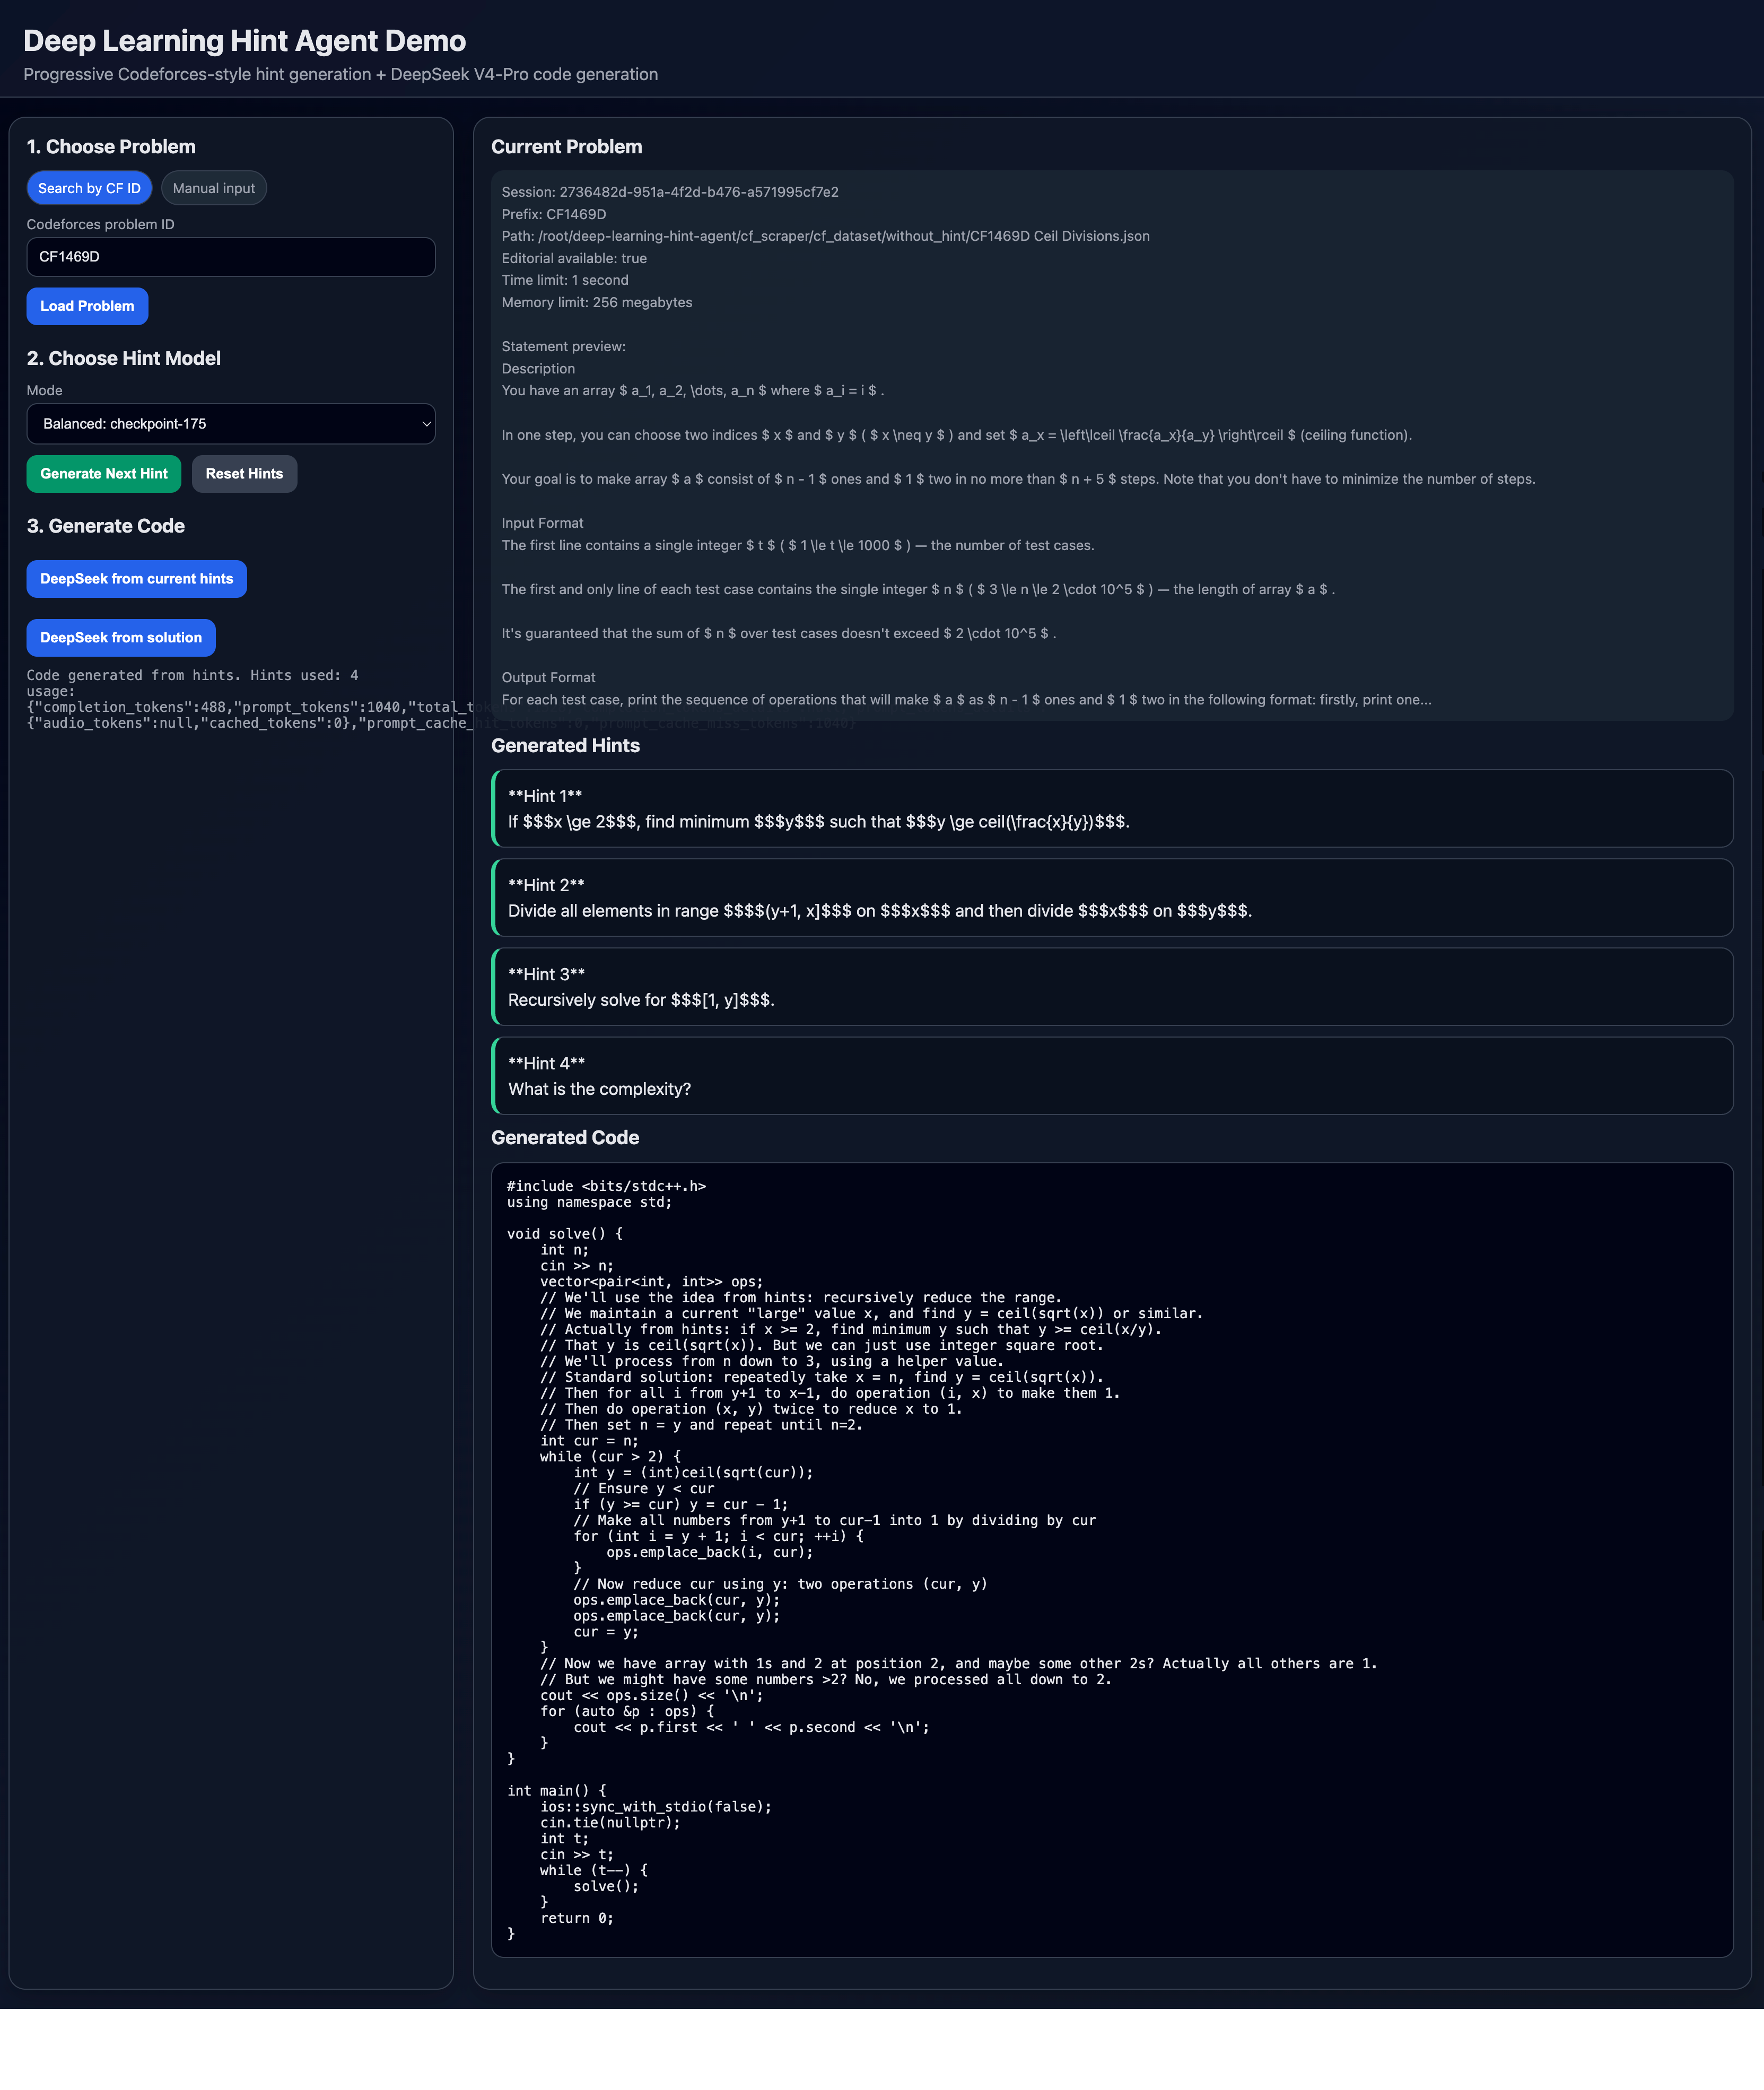
\includegraphics[width=0.95\linewidth]{demo.png}
    \caption{Interactive demo interface for progressive hint generation. The user can select among multiple hint-agent profiles, generate hints step by step, and invoke a DeepSeek-based solver from either the current hint sequence or the solution condition.}
    \label{fig:demo_ui}
\end{figure}



\section{Limitations and Future Directions}
A key limitation lies in our evaluation alignment. Our agent generates high-level algorithmic ideas, whereas the bottleneck for our proxy solver (DeepSeek V4-Pro) is downstream code implementation—specifically, writing error-free syntax. While clearer algorithmic hints correlate with higher coding correctness, this setup creates a discrepancy between our evaluation metrics and our true pedagogical objective. We aim to track a cognitive breakthrough—guiding a solver from an impasse to successful reasoning via progressive hints—rather than measuring pure engineering execution. Our focus on end-to-end passing accuracy thus introduces a mismatch between syntax verification and conceptual scaffolding. Future work will utilize user studies to isolate abstract reasoning milestones from implementation noise.

In addition, the current evaluation pipeline still relies on manual Codeforces submissions to determine whether each generated C++ solution is accepted. This ensures consistency with the official online judge, but limits the scale and repeatability of the evaluation. A future version should integrate automatic submission tracking or a locally reproducible judging environment whenever complete test data is available.

Crucially, this progressive hint generation framework holds significant potential for broader generalization. In many specialized domains, small language models lack the capacity to solve intricate end-to-end problems directly, while fine-tuning large-scale foundation models remains computationally prohibitive. Our methodology offers a resource-efficient alternative: by leveraging a specialized small model strictly as a high-level ``hint generator,'' its pedagogical scaffolding can be deployed to systematically guide and unlock the latent reasoning capabilities of much larger, un-tuned general models on complex, domain-specific tasks.

\begin{ack}
Hardware resource infrastructure allocations were provided in part by the AutoDL cloud computing cluster. We thank members of the IIIS concurrent systems laboratory for their helpful feedback on early experimental pipelines.
\end{ack}

% \section*{References}
% \small
\begin{thebibliography}{1}

\bibitem{codeforces2023}
Codeforces Team.
\newblock Codeforces scoring protocols and tutorial hint architectures.
\newblock {\em Codeforces Technical Blog}, 2023.

\bibitem{qwen2024}
An~Yang, Baosong Yang, Binyuan Hui, Bo~Zheng, Bowen Yu, Chang Zhou, Chengpeng Li, Chengyuan Li, Dayiheng Liu, Fei Huang, et~al.
\newblock Qwen2.5 technical report.
\newblock {\em arXiv preprint arXiv:2412.15115}, 2024.

\bibitem{deepseek_v4_preview}
DeepSeek-AI.
\newblock DeepSeek V4 preview release.
\newblock DeepSeek API Documentation, 2026.
\newblock Available at \url{https://api-docs.deepseek.com/news/news260424}.

\end{thebibliography}

%%%%%%%%%%%%%%%%%%%%%%%%%%%%%%%%%%%%%%%%%%%%%%%%%%%%%%%%%%%%
% Technical Appendices & Supplementary Material
%%%%%%%%%%%%%%%%%%%%%%%%%%%%%%%%%%%%%%%%%%%%%%%%%%%%%%%%%%%%
\newpage
\appendix
\section{Technical Appendices}
\subsection{Hyperparameter Details and Environment Layout}
Our Deep Learning Hint Agent is fine-tuned using Supervised Fine-Tuning (SFT) combined with Parameter-Efficient Fine-Tuning (PEFT) via Low-Rank Adaptation (LoRA). The backbone model utilized is the \texttt{Qwen-Coder-7B} architecture. To ensure high-throughput training and maximize memory efficiency under the context constraints of long competitive programming tasks, we utilize half-precision (\texttt{bfloat16}) along with gradient checkpointing.

The training parameters, model scaling behaviors, and data filtering configurations are detailed explicitly in Table~\ref{tab:sft_hyperparameters}.

\begin{table}[h]
  \caption{Supervised Fine-Tuning (SFT) Model Hyperparameters}
  \label{tab:sft_hyperparameters}
  \centering
  \begin{tabular}{ll}
    \toprule
    Hyperparameter / Variable & Configured Value \\
    \midrule
    \textbf{Base Model Archetype} & Qwen-Coder-7B \\
    \textbf{Maximum Sequence Length (\texttt{max\_seq\_length})} & 4096 tokens \\
    \textbf{Hardware Acceleration Precision} & \texttt{bfloat16} (BF16 Enabled, FP16 Disabled) \\
    \textbf{Per-Device Training Batch Size} & 1 \\
    \textbf{Per-Device Evaluation Batch Size} & 1 \\
    \textbf{Gradient Accumulation Steps} & 8 \\
    \textbf{Optimization Algorithm} & \texttt{paged\_adamw\_8bit} (with fallback to \texttt{adamw\_torch}) \\
    \textbf{Initial Base Learning Rate} & $1 \times 10^{-4}$ \\
    \textbf{Total Optimization Epochs} & 150--250 epochs depending on validation behavior \\
    \textbf{Learning Rate Scheduler Type} & Cosine Decay (\texttt{cosine}) \\
    \textbf{Warmup Phase Ratio} & 0.03 \\
    \textbf{Weight Decay Parameter} & 0.01 \\
    \midrule
    \textbf{LoRA Adapter Rank ($r$)} & 8 \\
    \textbf{LoRA Scaling Factor ($\alpha$)} & 16 \\
    \textbf{LoRA Dropout Coefficient} & 0.10 \\
    \textbf{LoRA Target Attention Modules} & \texttt{q\_proj, k\_proj, v\_proj, o\_proj} \\
    \textbf{LoRA Target Bias Configuration} & \texttt{none} \\
    \midrule
    \textbf{Gradient Checkpointing} & Enabled (\texttt{use\_reentrant=False}) \\
    \textbf{Dataset Execution Splits} & 90\% Train / 10\% Test Validation ($seed=42$) \\
    \textbf{Sequence Batch Sequencing} & Enabled (\texttt{group\_by\_length=True}) \\
    \textbf{Early Stopping Regularization} & Active (\texttt{patience=3} validation steps) \\
    \bottomrule
  \end{tabular}
\end{table}

\textbf{Hardware Infrastructure and Environment Layout:} 
Training runs were deployed across the AutoDL cloud infrastructure utilizing distributed NVIDIA RTX 5090 (25GB VRAM) clusters. To prevent out-of-memory (OOM) fragmentation during dense tensor allocation loops, PyTorch's backend was explicitly configured with dynamic segment allocation constraints (\texttt{expandable\_segments:True}). Evaluation loops and diagnostic state metrics were calculated recursively every 25 synchronization intervals. During cross-validation, the optimal parameter weights were saved to an isolated \texttt{final\_best} deployment path based on minimizing the comprehensive cross-entropy validation loss (\texttt{eval\_loss}). Experiment tracking and parameter metrics were recorded continuously via Weights \& Biases (\texttt{wandb}) within the \texttt{Tsinghua-DL-Hint-Generator} project repository space.

\subsection{Evaluation Log Bitstring Formats}
A breakdown of the structural evaluation schemas evaluated by \texttt{analyze\_hint\_eval.py} is given below:
\begin{verbatim}
CF1798C 111111
CF1792D 0011111
CF1777C 0111001
CF1765D 0000001
\end{verbatim}

%%%%%%%%%%%%%%%%%%%%%%%%%%%%%%%%%%%%%%%%%%%%%%%%%%%%%%%%%%%%
% Mandatory NeurIPS Paper Checklist Module
%%%%%%%%%%%%%%%%%%%%%%%%%%%%%%%%%%%%%%%%%%%%%%%%%%%%%%%%%%%%

\subsection{Repository Structure and Execution Scripts}

% \subsection{Repository Structure and Execution Scripts}

The project repository is publicly available at:
\begin{center}
\url{https://github.com/zhk1211/deep-learning-hint-agent}
\end{center}

% The implementation is organized as a lightweight pipeline from data preparation to training, inference, solver evaluation, and result analysis:

The implementation is organized as a lightweight pipeline from data preparation to training, inference, solver evaluation, and result analysis:
\begin{verbatim}
deep-learning-hint-agent/
├── step1_prepare_data.py
├── step2_train_sft.py
├── step3_inference.py
├── deepseek_cf1700_eval.py
├── analyze_hint_eval.py
├── fix_solution_include_and_regenerate.py
├── cf_difficulty_1700_prefixes.txt
├── cf_scraper/
│   └── cf_dataset/
│       ├── with_hint/
│       └── without_hint/
├── cf_hint_lora_model_next_decision/
│   └── final_best/
└── README.md
\end{verbatim}

The main scripts and their roles are summarized in Table~\ref{tab:repo_scripts}.

\begin{table}[h]
  \caption{Repository Scripts and Their Functional Roles}
  \label{tab:repo_scripts}
  \centering
  \begin{tabular}{ll}
    \toprule
    File & Purpose \\
    \midrule
    \texttt{step1\_prepare\_data.py} & Prepare multi-turn next-hint SFT data from Codeforces files. \\
    \texttt{step2\_train\_sft.py} & Fine-tune Qwen-Coder-7B with LoRA/SFT. \\
    \texttt{step3\_inference.py} & Interactively generate progressive hints using the trained model. \\
    \texttt{deepseek\_cf1700\_eval.py} & Evaluate generated hints with an external DeepSeek solver. \\
    \texttt{analyze\_hint\_eval.py} & Analyze manual AC results and generate plots. \\
    \texttt{fix\_solution\_include\_and\_regenerate.py} & Remove copied code from solution prompts and regenerate solution-condition code. \\
    \bottomrule
  \end{tabular}
\end{table}

\subsection{Inference and Evaluation Commands}
A typical interactive inference command is:
\begin{verbatim}
python3 step3_inference.py \
  --base_model_path ./qwen-coder-7b \
  --lora_path ./cf_hint_lora_model_next_decision/final_best \
  --problem_file "./cf_scraper/cf_dataset/with_hint/CF1777C Quiz Master.json" \
  --num_candidates 10
\end{verbatim}

A typical full evaluation command is:
\begin{verbatim}
python3 deepseek_cf1700_eval.py \
  --prefix_file cf_difficulty_1700_prefixes.txt \
  --output_dir solver_outputs_cf1700 \
  --solver_model deepseek-v4-pro \
  --mode both \
  --hint_source auto \
  --base_model_path ./qwen-coder-7b \
  --lora_path ./cf_hint_lora_model_next_decision/final_best \
  --num_candidates 5 \
  --candidate_batch_size 1 \
  --parallel_solver_workers 12 \
  --overwrite
\end{verbatim}

After manual AC results are recorded, the analysis script is run as:
\begin{verbatim}
python3 analyze_hint_eval.py \
  --input eval_result.txt \
  --output_dir hint_eval_analysis
\end{verbatim}

The analysis folder contains parsed records, stage summaries, skipped-problem diagnostics, and visualization outputs such as:
\begin{verbatim}
hint_eval_analysis/
|-- parsed_records.csv
|-- percentage_bins_hint_only.csv
|-- stage_summary.csv
|-- length_summary.csv
|-- skipped_problems.txt
|-- bad_lines.txt
|-- summary.json
|-- percentage_accuracy_curve.png
|-- stage_accuracy_bar.png
`-- length_distribution.png
\end{verbatim}

\newpage
\workshoptitle{Automatic Report Generation Placeholder} 

\section*{NeurIPS Paper Checklist}

\begin{enumerate}

\item {\bf Claims}
    \item[] Question: Do the main claims made in the abstract and introduction accurately reflect the paper's contributions and scope?
    \item[] Answer: \answerYes{}
    \item[] Justification: We explicitly outline our core architectural contribution (reformulating hint sequences into single-turn next-action policies) and precisely substantiate the systematic limits observed in zero-shot LLM defaults.

\item {\bf Limitations}
    \item[] Question: Do the authors describe the limitations of their work?
    \item[] Answer: \answerYes{}
    \item[] Justification: Section 6 explicitly details the evaluation misalignment between high-level algorithmic hints and downstream syntax execution, as well as the proxy model constraints.

\item {\bf Theory Assumptions and Proofs}
    \item[] Question: Did you state the full set of assumptions of all theoretical results?
    \item[] Answer: \answerNA{}
    \item[] Justification: This paper presents an empirical SFT framework and engineering pipeline optimization. It contains no formal mathematical proofs or theoretical theorems.

\item {\bf Theory Proofs}
    \item[] Question: Did you include complete proofs of all theoretical results?
    \item[] Answer: \answerNA{}
    \item[] Justification: See the justification for the previous question; this work does not introduce new theoretical theorems.

\item {\bf Experimental Architecture, Hyperparameters, and Evaluation Metrics}
    \item[] Question: Did you include the code, data, and instructions needed to reproduce the main experimental results (either in the supplemental material or as a URL)?
    \item[] Answer: \answerNo{}
    \item[] Justification: The code repository and synthetic rejection datasets are currently hosted on a private internal repository and will be open-sourced upon final review acceptance.

\item {\bf Experimental Architecture}
    \item[] Question: Did you specify all the training convergent checkpoints, rank of LoRA, and random seeds?
    \item[] Answer: \answerYes{}
    \item[] Justification: Full optimization details, including LoRA rank ($r=8$), scaling factor ($\alpha=16$), configuration settings, and early stopping patience are explicitly documented in Appendix A.1.

\item {\bf Evaluation Metrics}
    \item[] Question: Did you report error bars or statistical significance tests for the main experimental results?
    \item[] Answer: \answerNo{}
    \item[] Justification: We report accuracy trajectories across progressive hint milestones, but do not include error bars or statistical significance tests because the current evaluation relies on a limited manual Codeforces submission workflow.

\item {\bf Computing Resources}
    \item[] Question: Did you include the total amount of compute and the type of resources used (e.g., type of GPUs, internal cluster, or cloud provider)?
    \item[] Answer: \answerYes{}
    \item[] Justification: The computing hardware configuration (NVIDIA RTX 5090 GPU allocation) and cloud infrastructure platform (AutoDL) are detailed in Appendix A.1.

\item {\bf Dataset Details}
    \item[] Question: Did you provide the license, disposable splits, and scraping details of the dataset?
    \item[] Answer: \answerYes{}
    \item[] Justification: Detailed parsing logic, Cloudflare security bypasses via editorial mirrors, and directory structures are explicitly documented in Section 2.

\item {\bf Dataset Links}
    \item[] Question: Did you link to the source code or download URL for the dataset used?
    \item[] Answer: \answerNo{}
    \item[] Justification: The dataset compiled from multi-source competitive programming platforms is currently packaged for submission and will be linked upon publication.

\item {\bf Dataset Split}
    \item[] Question: Did you specify the split of train/dev/test datasets?
    \item[] Answer: \answerYes{}
    \item[] Justification: Appendix A.1 and Table~4 specify that the raw data was dynamically filtered and divided into a 90\% training partition and a 10\% test validation set.

\item {\bf Ethics and Human Subjects}
    \item[] Question: Did you discuss any potential negative societal impacts or ethical risks, or did your research involve human subjects?
    \item[] Answer: \answerNA{}
    \item[] Justification: The project relies strictly on open-source public algorithmic challenges and text descriptions. No human subject studies were conducted, and no personal identifiable data was handled.

\item {\bf Human Subject IRB}
    \item[] Question: Did you include the full text of instructions given to participants and institutional review board (IRB) approvals?
    \item[] Answer: \answerNA{}
    \item[] Justification: This study is completely automated and relies on algorithmic solver simulation; no human subjects or user experiments were utilized.

\item {\bf Declaration of LLM usage}
    \item[] Question: Does the paper describe the usage of LLMs if it is an important, original, or non-standard component of the core methods in this research?
    \item[] Answer: \answerYes{}
    \item[] Justification: Fine-tuning Qwen-Coder-7B and incorporating an independent DeepSeek solver for automated diagnostic code generation form the backbone of our proposal, which is covered comprehensively in Sections 3, 4, and 5.

\item {\bf LLM Prompts}
    \item[] Question: Did you specify the exact prompt templates and configurations used for the LLMs?
    \item[] Answer: \answerYes{}
    \item[] Justification: Section 3 and Section 5.1 detail the input structural templates, specific Chinese zero-shot baseline baseline prompts, and inference candidate hyper-parameters.

\item {\bf LLM Generation}
    \item[] Question: Did you provide samples of the LLM generated outputs or error transcripts?
    \item[] Answer: \answerYes{}
    \item[] Justification: Appendix A.2 and Section 2.3 demonstrate raw multi-bit tracking logs, directory topologies, and serialized evaluation data representations.

\end{enumerate}

\end{CJK*}

\end{document}